\chapter{Análise Bibliográfica sobre Riscos em Crédito Bancário e Sistemas Inteligentes Antifraude, por Lucas Gurgel\label{chap:bibliometria:lggurgel}}

\section{Planejamento do estudo}
Os principais bancos e instituições financeiras estão se adaptando cada dia mais às novas necessidades tecnológicas de seus clientes e muito dos serviços que antes havia certa burocracia para se concluírem, hoje são realizados boa parte virtualmente e, em muitos casos, complatamente remota.
Esse estudo pretende descrever quais as frentes de pesquisa científica que estudam métodos para se evitar fraudes e inadimplência. 
O planejamento inicial do estudo pretende trazer respostas para as seguintes questões:

\begin{itemize}
    \item Qual a base de conhecimentos científicos produzida em torno do tema análise de crédito bancário oferecido à interessados utilizando sistemas computacionais para evitar fraudes e inadimplências? 
    \item Como os sistemas computacionais ajudam nas decisões das grandes instituições financeiras a reduzirem o risco ao ceder crédito ao consumidor?
    \item Quais os principais termos e conceitos ligados à frente de pesquisa relacionado ao tema análise de crédito que utilizam sistemas computacionais?
    \item Quais são os primeiros interessados em estudar esse tema e aplicá-lo no meio social?
\end{itemize}

\subsection{Uso do Bibliometrix e Biblioshiny}
A análise será realizada pelo uso da plataforma R e ferramenta e fluxo de análise \textit{workflow} proposto pelos autores do pacote Bibliometrix, conforme indica a figura ~\ref{fig:bibliometrix:workflow}.

\subsection{Limitações} O exercício relatado foi feito em três dias, envolvendo entre 12 a 15 horas de trabalho do autor.

\section{Coleta de dados\label{RCBSIA:coleta}}

A coleta de dados foi realisada usando base de dados Web of Science no dia 7 de fevereiro de 2022, acessado por meio do Portal de Periódicos da CAPES.

Foram feitas buscas nas coleções \textbf{Science  Citation  Index  Expanded (SCI -EXPANDED)} e \textbf{Social  Sciences  Citation  Index (SSCI)}, que contém registros relativos a vários campos do conhecimento, no qual o SCI-EXPANDED foca mais na área das ciências exatas e naturais, enquanto que o SSCI indexa artigos da área das ciências sociais. Importante observar que os artigos nessas duas coleções são indexados desde o ano de 1945. 

\subsection{Query de Busca}

Foi usada a \query\  de busca ilustrada nas linhas 1 a 11 da listagem \ref{query20220207}.

\lstinputlisting[numbers=left,basicstyle=\normalsize\ttfamily,caption={\query\  de busca sobre riscos em crédito bancário, com ênfase em sistemas inteligentes antifraude.},label=query20220207]
{experiments/lggurgel/AnaliseBibliometrica/RiscoBancario/WoS-20220207/query.txt}

\subsubsection{Explicação para os termos de busca usados\label{RCBSIA:query}}

A busca foi construída acerda de declarações disjuntivas \textit{or} e conjuntivas \textit{and}. A busca permitiu buscar temos charve nas seguintes estuturas dos artigos:
\begin{itemize}
    \item Título 
    \item Resumo (Abstract)
    \item Author Keywords
    \item Keywords Plus da referência
\end{itemize}

Os termos \texttt{experimental}, \texttt{analy*} e \texttt{model*}, (linha 1 da query) foram usados na primeira cláusula da \query\  para recuperar artigos que tenham em seu título, palavras-chave e resumo, termos relacionados a métodos experimentais,
métodos analíticos e métodos de modelagem.

O termo \texttt{bank*}, na linha 3, foi usado em conjunção com os demais para recuperar apenas trabalhos que explicitem estudos voltados somente para bancos ou operações bancárias.

A cláusula  na linha 5, faz união entre o uso dos termos \texttt{risk}, \texttt{fraud} e \texttt{fake}, para cobrir estudos que tem por interesse os riscos banários, falsificações bancárias e principalmente risco bancário.

A cláusula  na linha 7, também faz uma união. O uso dos termos \texttt{lending} e \texttt{loan}, \texttt{credit}, \texttt{pay*} e também \texttt{delinquency}, é utilizado para cobrir as principais operações e processos sofridos e realizados pelas organizações interessadas do estudo.

A última cláusula, usou os termos \texttt{software}, \texttt{algorithm} e \texttt{tech*}, para recuperar artigos que tratem de soluçoes tecnológicas acerca do tema.

\subsection{Registros recuperados}

Foram obtidos no total 3.628 registros como resultado da busca, disponível em \url{https://github.com/jhcf/Comput-Experim-20212/experiments/lggurgel/AnaliseBibliometrica/RiscoBancario/WoS-20220207/savedrecs3628.txt}. 


\section{Análise dos dados}

\subsection{Filtragem de registros}
Antes da análise, é possível aplicar filtros sobre os registros obtidos.

Foi aplicado um filtro ao \dataset\   inicial, com 3.628 registros, que continham pŕevias de artigos, artigos de conferência, capítulos de livro etc. Foram mantidos apenas os registros de artigos publicados em revistas científicas\footnote{A suposição é que que o conhecimento de maior qualidade sobre o tema está nas publicações em revistas.}. Após a aplicação desse filtro, 2.213 registros foram mantidos no \dataset, que será de agora em diante referenciado por RCBSIA@lggurgel.

\subsection{Análise descritiva do \dataset\   RCBSIA@lggurgel}

A análise bibliométrica descritiva do \dataset\ foi gerada pela função \texttt{biblioAnalysis}.

As informações mais gerais sobre o \dataset\   RCBSIA@lggurgel são as seguintes:
\begin{description}
    \item [\textit{Timespan}] Os artigos que atenderam aos critérios de busca e filtragem foram publicados a partir de 1989, até 2021.
    \item [\textit{Sources (Journals, Books, etc)}] São 840 fontes de informação que publicaram os documentos recuperados no \dataset\. Ou seja, em média, cada \textit{scientific journal} publicou $2.213/840=2,6$ artigos.
    \item [\textit{Average years from publication}] A média do tempo de publicação dos artigos no \dataset\   RCBSIA@lggurgel é de 5,45 anos.
    \item [\textit{Average citations per documents}] Cada artigo no \dataset\   RCBSIA@lggurgel foi citado, em média 23,46 vezes.
    \item [\textit{Average citations per year per doc}] Após publicado, cada um dos 2.213 artigos do \dataset\  foi citado 3,092 vezes por ano, em média.
    \item [\textit{References}] O \dataset\   RCBSIA@lggurgel contém 70.466 referências citadas (tags CR).
    \item [\textit{Keywords Plus (ID)}] 3.217 distintas palavras-chave do tipo Keywords Plus (ID)\footnote{\textit Termos de índice gerados automaticamente a partir dos títulos de artigos citados.}
    \item [\textit{Author's Keywords (DE)}] 6.098 distintas palavras-chave indicadas pelos autores foram encontradas no \dataset\  .
    \item [\textit{Authors}] 22.205 distintos nomes de autores foram encontrados no \dataset\ .
    \item [\textit{Authors of single-authored documents}] Dentre os 22.205 distintos (nomes de) autores encontrados, 265 deles editaram artigos individualmente.
    \item [\textit{Authors of multi-authored documents}] Dentre os 22.205 distintos autores encontrados, 21.940 deles editaram artigos com um ou mais co-autores"
    \item [\textit{Single-authored documents}] Dentre os 2.213 documentos presentes no \dataset\ , 294 foram escritos por um único autor.
    \item [\textit{Documents per Author}] Dentre os 22.205 distintos (nomes de) autores, cada um publicou em média 0,0997 artigos.
    \item [\textit{Authors per Document}] Cada um dos 2.213 documentos presentes no \dataset\ foi autorado com 10 autores em média.
    \item [\textit{Co-Authors per Documents}] As 42.161 aparições de (nomes de) autores (``Author Appearances''), sem distribuem, em média 19,1 vezes para os 2.213 documentos do \dataset\   RCBSIA@lggurgel.
    \item [\textit{Collaboration Index}] Os 42.161 autores que editaram artigos com um ou mais co-autores, colaboraram em media 11,4 vezes para editar os 2.213 artigos elaborados em co-autoria.
\end{description}

\subsection{Evolução da Produção Científica}

\begin{figure}
    \centering
    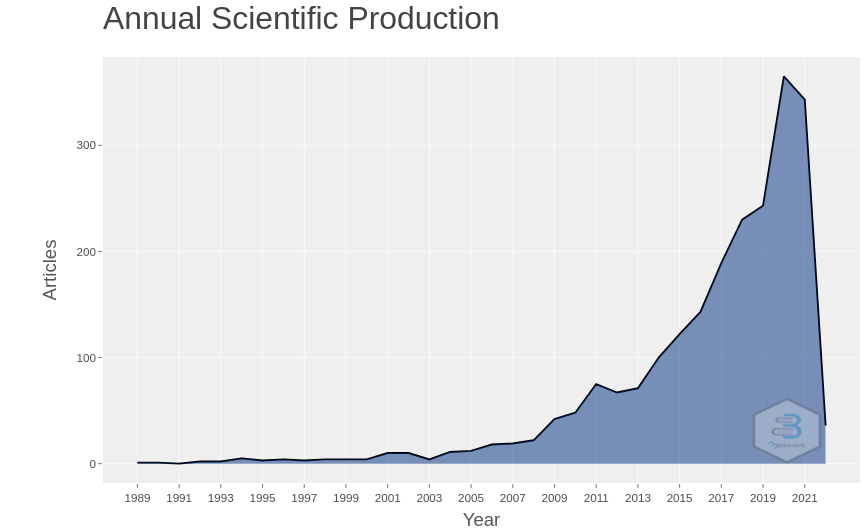
\includegraphics[width=1\textwidth]{experiments/lggurgel/AnaliseBibliometrica/RiscoBancario/Figs/Descritiva/RCBSIA-ProducaoCientificaAnual.png}
    \caption{Evolução da produção científica anual no \dataset\   RCBSIA@lggurgel.}
    \label{fig:evol:anual:RCBSIA@lggurgel}
\end{figure}

A figura \ref{fig:evol:anual:RCBSIA@lggurgel} apresenta a evolução da produção científica mundial no tema Riscos em Crédito Bancário e Sistemas Inteligentes Antifraude, segundo o \dataset\   RCBSIA@lggurgel. A curva mostra uma tendência de crescimento aproximadamente exponencial da quantidade de publicações, desde a primeira identificada em 1989.

\subsection{Interpretação do Crescimento} A taxa de crescimento do \dataset\   RCBSIA@lggurgel sugere que o assunto em pauta despertou intenso interesse no ano de 2004 e desde então aumentou significamente. Isso se deu pelo fato de grandes bancos internacionais na China e Estados Unidos, principalmente, focarem seus investimentos em tecnologias e soluções para os problemas de fraudes e redução de risco.

\subsection{Evolução das Citações}

\begin{figure}
    \centering
    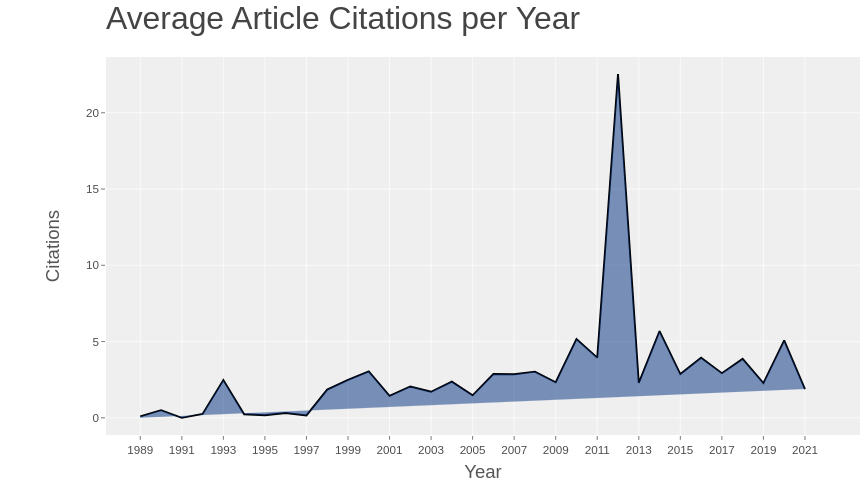
\includegraphics[width=1\textwidth]{experiments/lggurgel/AnaliseBibliometrica/RiscoBancario/Figs/Descritiva/RCBSIA-MediaAnualCitacoes.png}
    \caption{Evolução das citações ao \dataset\   RCBSIA@lggurgel.}
    \label{fig:evol:anual:citacoes:RCBSIA@lggurgel}
\end{figure}

A figura \ref{fig:evol:anual:citacoes:RCBSIA@lggurgel} apresenta a evolução da média de citações aos 2.213 artigos no \dataset\   RCBSIA@lggurgel. 
Nota-se uma estabilidade na média anual de citações, onde os artigos publicados em 1989 até os dias atuais com cerca de 2 a 5 citações médias, e em 2011-2012 o valor médio divergiu para quase 30 citações. Esse pico deve-se à presença de um artigo do \dataset que possui um número surpreendente grande de citações.

\subsection{Interpretação das Citações}
Mesmo perante um crescimento aproximadamente exponencial no volume de publicações, a ocorrência de um crescimento nas citações médias ao longo dos anos sugere que os artigos do \dataset\   possuem uma tendência de crescimento no tamanho da bibliografia citada, bem como também despertam grande interesse dos cientistas nas demais áreas do conhecimento.

\subsection{\textit{Three-Field Plots (Sankey diagram)} \label{RCBSIA:Sankey}}

As \textit{Three-Field Plots (Sankey diagram)} (plotagens do tipo ``Três Campos'') apresentam afinidades entre três conjuntos de atributos agregados que ocorrem no \dataset, que busca mostrar os principais fluxos entre alguns conjuntos de itens.

\begin{figure}
    \centering
    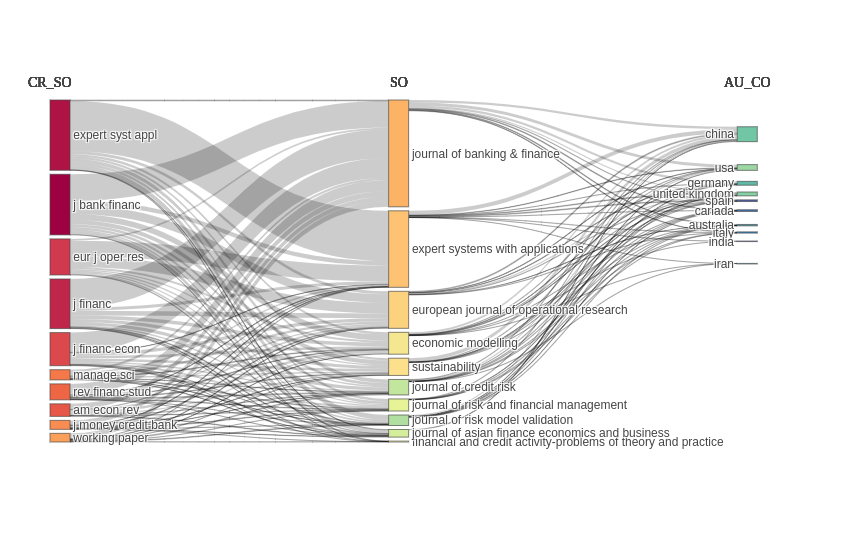
\includegraphics[angle=0,width=1\textwidth]{experiments/lggurgel/AnaliseBibliometrica/RiscoBancario/Figs/Descritiva/RCBSIA-GraficoArvore-CR_SO-SO-AU_CO.png}
    \caption{Plotagem ``Três Campos'' (Sankey plot) do \dataset\   RCBSIA@lggurgel: 10 Referências, Fontes e Países mais envolvidos.}
    \label{fig:RCBSIA@lggurgel:ThreeFieldPlot}
\end{figure}

A figura \ref{fig:RCBSIA@lggurgel:ThreeFieldPlot} representa a plotagem do tipo ``Três Campos'' do \dataset\   RCBSIA@lggurgel. No centro, as 10 fontes mais proeminentes (SO), à esquerda, as 10 Citações mais frequentes (CR - Cited Records), e à direita, os 10 países mais frequentes originantes dos estudos.

\subsection{Interpretação da figura \ref{fig:RCBSIA@lggurgel:ThreeFieldPlot}}

As dez referências mais relevantes, citados pelos artigos do \dataset\ RCBSIA, possuem relações com as principais fontes dos artigos e vice-versa. É possivel notar também a diversidade de países que abordam o tema, com destaque à China.

Adicionalmente, dentre as palavras-chave (DE) não relacionadas diretamente aos termos de busca, emergem os termos \textbf{distributed control}, \textbf{event-triggered control}, \textbf{consensus} e \textbf{opinion dynamics}. Isso sugere foco das pesquisas por autores de origem chinesa no uso de simulação multiagente voltada à compreensão dos fenômenos de controle social distribuído, formação de consenso e dinâmica da opinião (pública?).

Ainda sobre a interpretação da plotagem da figura \ref{fig:RCBSIA@lggurgel:ThreeFieldPlot}, observa-se que os artigos mais citados encontram-se publicados pelo menos 10 anos atrás, sugerindo que não houve, nos últimos 10 anos, nenhum trabalho que tenha produzido uma mudança de paradigma no tema.
A fim de melhor evidenciar as citações mais relevantes segundo o peso das referências e países, o gráfico da figura \ref{fig:RCBSIA@lggurgel:ThreeFieldPlot2} plota apenas as 10 referências citadas, para 20 autores e palavras-chave mais proeminentes.

\begin{figure}
    \centering
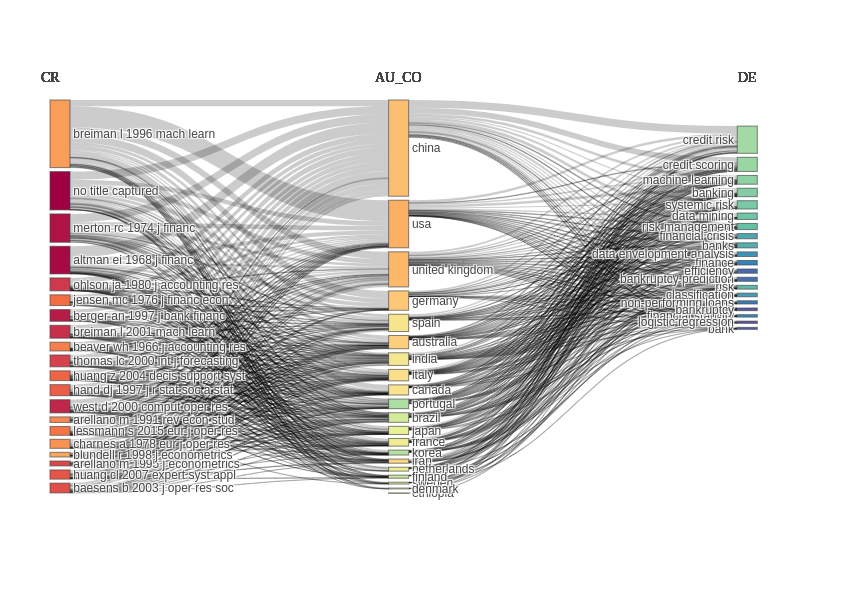
\includegraphics[angle=0,width=1\textwidth]{experiments/lggurgel/AnaliseBibliometrica/RiscoBancario/Figs/Descritiva/RCBSIA-GraficoArvore-CR-AU_CO-DE.png}
    \caption{Plotagem ``Três Campos'' (Sankey plot) do \dataset\   RCBSIA@lggurgel: 10 maiores Referências Citadas, 10 Países e Palavras-Chave mais predominantes.}
    \label{fig:RCBSIA@lggurgel:ThreeFieldPlot2}
\end{figure}

\begin{figure}
    \centering
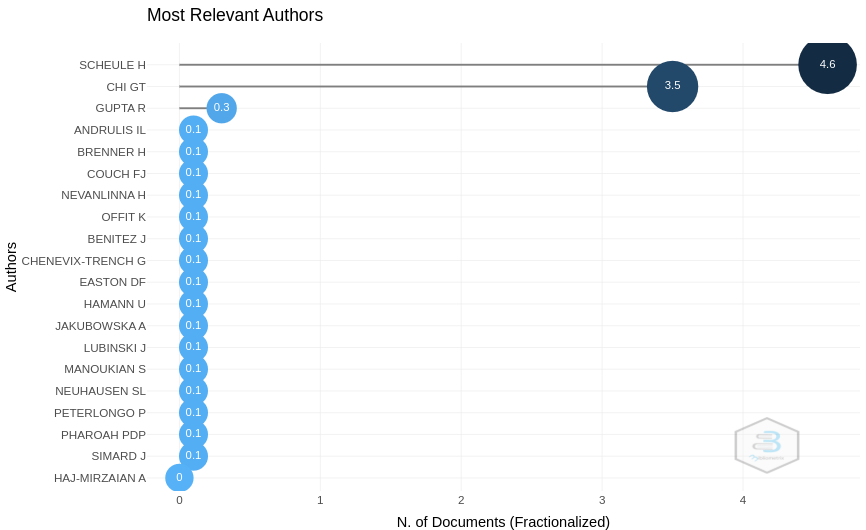
\includegraphics[angle=0,width=1\textwidth]{experiments/lggurgel/AnaliseBibliometrica/RiscoBancario/Figs/Descritiva/RCBSIA-AutoresRelevantes.png}
    \caption{Autores mais relevantes responsáveis por liderarem os principais estudos do \dataset RCBSIA@lggurgel.}
    \label{fig:RCBSIA@lggurgel:RelevantAuthors}
\end{figure}

\begin{figure}[htp]
    \centering
    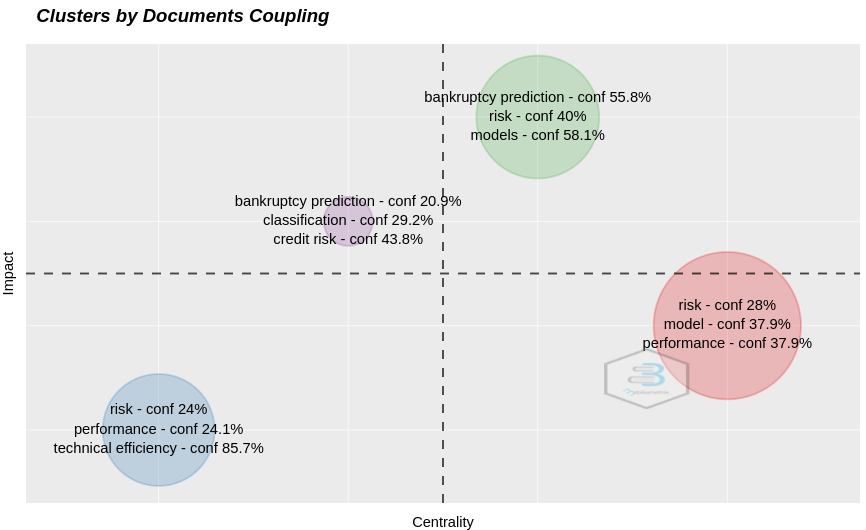
\includegraphics[angle=0,width=1\textwidth]{experiments/lggurgel/AnaliseBibliometrica/RiscoBancario/Figs/Metricas/RCBSIA-ClusterDocumentos.png}
    \caption{Rede de co-ocorrência de palavras, com 150 termos, aplicada ao \dataset\   RCBSIA@lggurgel.}
    \label{fig:RCBSIA@lggurgel:redecoocorr}
\end{figure}

As seguintes palavras foram identificadas nesse \textit{cluster}:
risk,
model,
performance,
bankruptcy prediction,
credit risk e
technical efficiency. 

